\chapter{Modeling Local Particulate Matter Dynamics with Time Delay Embeddings}\label{ch:havok}
% \chapter{Time-delay Embedding Models for Particulate Matter - Outlier Detection and Forecasting}\label{ch:havok}

\textcolor{magenta}{Should we keep the variogram stuff?}


The low-cost sensor network detailed in Chapter~\ref{ch:air-network} collects a
continuous stream of air quality data for a plethora of locations with high
temporal resolution ranging between $0.1$ to $1.0$ Hz. The real-time
visualization dashboards developed for the network offer immediate insight into
local air conditions. However, the challenge remains to extract actionable
insights from the large amounts of historical data. For example, we are concerned
with answering simple questions such as: \textit{What is the typical pattern of
  PM variability at this location}, \textit{Are changes in PM gradual or due to
  identifiable events?}, and \textit{Can we use historical PM measurements to
  provide insight into future air quality trends?}.

In this chapter, we propose a physics-based model rooted in Koopman operator
theory to address these questions by accurately capturing local PM dynamics.
Specifically, we extend the \textit{Hankel Alternative View of Koopman} (HAVOK)
framework introduced by Brunton et al. to apply to time series measurements of
PM data. In this data-driven approach PM dynamics are described via a simple
linear system with aperiodic external forcing. The forcing function extracted
from the model provides a clear method to identify abrupt pollution events from
historical data. The model can be used to provide accurate short-term forecasts.
Importantly, HAVOK models require few parameters, can be fit efficiently using
established numerical linear algebra routines, and are small enough to be
readily deployed directly onto sensor hardware.


\section{Motivation}


% Particulate matter (PM) dynamics exhibit complex behavior influenced by a variety of factors, including meteorological conditions, human activities, and atmospheric processes. PM concentrations typically follow well-established diurnal patterns, with peaks often occurring during morning and evening rush hours due to increased vehicular emissions, and lower concentrations observed during the midday when atmospheric dispersion is more effective (Zhang et al., 2012). Seasonal variations are also common, with higher PM levels in winter due to factors like heating emissions and temperature inversions that trap pollutants close to the ground (Cheng et al., 2013). Numerous models have been developed to analyze and forecast PM levels. These range from statistical models, such as autoregressive integrated moving average (ARIMA) models (Box et al., 1994), to more sophisticated machine learning approaches like neural networks, which can capture nonlinear relationships in the data (Zhang et al., 2020). Physics-based models, including chemical transport models (CTMs), provide detailed representations of atmospheric processes but require substantial computational resources and detailed input data (Seinfeld & Pandis, 2016). More recently, hybrid approaches combining machine learning with physical models have shown promise in improving forecast accuracy by leveraging the strengths of both methodologies (Bi et al., 2021). 

% ---

% **References:**

% 1. Zhang, Y., et al. (2012). "Diurnal variation in PM2.5 concentration and its causes." *Atmospheric Environment*, 45(8), 2017-2024.
% 2. Cheng, Y., et al. (2013). "Wintertime PM2.5 variations in China." *Environmental Pollution*, 182, 44-51.
% 3. Box, G.E.P., et al. (1994). *Time Series Analysis: Forecasting and Control*. Prentice Hall.
% 4. Zhang, Z., et al. (2020). "Air quality prediction using machine learning methods." *Journal of Environmental Management*, 242, 465-473.
% 5. Seinfeld, J.H., and Pandis, S.N. (2016). *Atmospheric Chemistry and Physics: From Air Pollution to Climate Change*. John Wiley & Sons.
% 6. Bi, J., et al. (2021). "A hybrid approach for PM2.5 forecasting: Combining physics-based models with deep learning." *Environmental Modelling & Software*, 139, 105014.



- Dynamics of particulate matter


- Time series models for PM (how good are forecasts)


- Value of a physics-based models, e.g. chemical transport

- Limitations of these models are due to poorly resolved meteorological
obsevations, for example, high resolution ECMWF analysis are at 0.1 x 0.1 km
grids with the lowest vertical model layer hundreds of meters above the ground.

- Many of these are being developed but have yet to see application to
realistic, noisy datasets




It should be noted that
despite the rapid pace of development in the fields of data-driven and
scientific machine learning, many recently developed techniques like the
Universal Differential Equations (UDEs), Hamiltonian Neural Networks, and others
have yet to see wide spread application on noisy, real-world datasets. Our
secondary goal for this chapter is therefore to demonstrate how, with some
slight modifications, these techniques can be applied to real-world problems.


In order to provide actionable insights we must be able to effectively model the
dynamics of our collected time series. In a perfect world, we would measure all
relevant physical quantities such that the time evolution of local air quality
at each sensor could be obtained by simulating the relevant micro-physics.
However, low cost sensor networks are not equipped with all the necessary
reference grade instruments needed to perform such simulations; accurate winds
speed and direction sensors alone can cost hundreds to thousands of dollars and
remote sensing data products are often unreliable at the ground level (i.e. in
the human head space). We therefore are motivated to develop techniques to model
our collected time series using only the data provided at a single node. There
are many approaches to this task in the statistics and machine learning
literature including statistical models like ARIMA and deep learning methods
like Recurrent Neural Networks \cite{intro-to-time-series-models,
  time-series-rnns}. While these methods can often lead to robust short term
predictions, they do not incorporate prior physics knowledge and therefore are
not primed to take advantage of underlying dynamical laws. Recently two
interesting physics-informed, data driven techniques have been developed for
just this type of scenario. The first we shall examine is the so-called
\textit{Hankel Alternative View Of Koopman} (HAVOK) framework which extends the
principle of dynamic mode decomposition to nonlinear systems
\cite{brunton-havok}. The second is an technique dubbed the \textit{Hamiltonian
  Neural Network} which extends the notion of a Neural Ordinary Differential
Equation to allow a neural network to learn coordinate transformations or the
original time series data which satisfy \textit{Hamiltons equations}
\cite{greydanus-hnn}.




Note the additional constraint that our model should be both physically
interpretable and small enough to be easily trained and deployed at scale. While
complicated DNN based approaches such as deep recurrent networks may provide an
ability to forecast, the size and training times involved for these approaches
are prohibitively high if we wish to train and deploy these models directly to
sensors in the network in an automated fashion. Also note the other HAVOK paper
which attempts to use HAVOK for predictions which showed that the HAVOK model
provides a superior one step prediction compared to other state of the art
models.


\section{Hankel Alternative View of Koopman}

\subsection{Koopman Operator Theory}

\subsection{Time-Delay Embeddings and Taken's Theorem}

\subsection{Hankel Alternative View of Koopman}


\subsection{Simple Example: Lorenz System}


\begin{figure}[h]
  \centering
  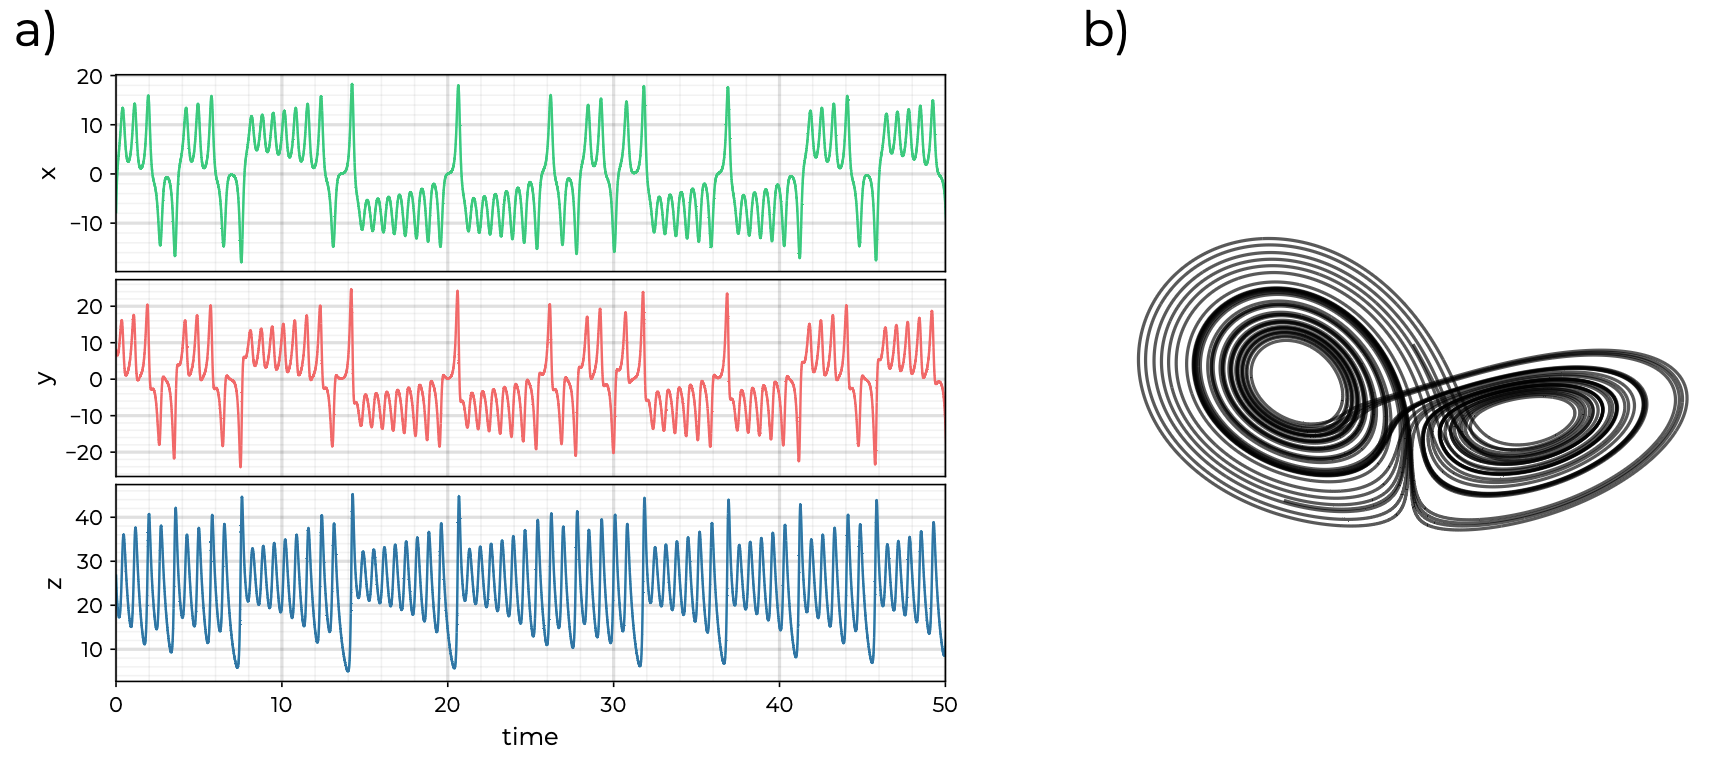
\includegraphics[width=\columnwidth]{havok/0-havok-lorenz/2__lorenz-orig.png}
  \caption{(\textbf{a}) Time series for the $x$, $y$, and $z$ components of the
    Lorenz system. (\textbf{b}) 3-dimensional visualization of the attractor
    formed from $x$, $y$, and $z$ components. We note that there are two clear
    lobes corresponding to the two attractors of the system.}
  \label{fig:lorenz-time-series-orig}
\end{figure}


\begin{figure}[h]
  \centering
  \includegraphics[width=0.5\columnwidth]{havok/0-havok-lorenz/1b_A-B-sHAVOK.pdf}
  \caption{Fitted operators $\mathbf{A}$ and $\mathbf{B}$ for the Lorenz system
    learned by the HAVOK model corresponding to the linear dynamics and
    intermittent forcing.}
  \label{fig:lorenz-A-B-heatmap}
\end{figure}


\begin{figure}[h]
  \centering
  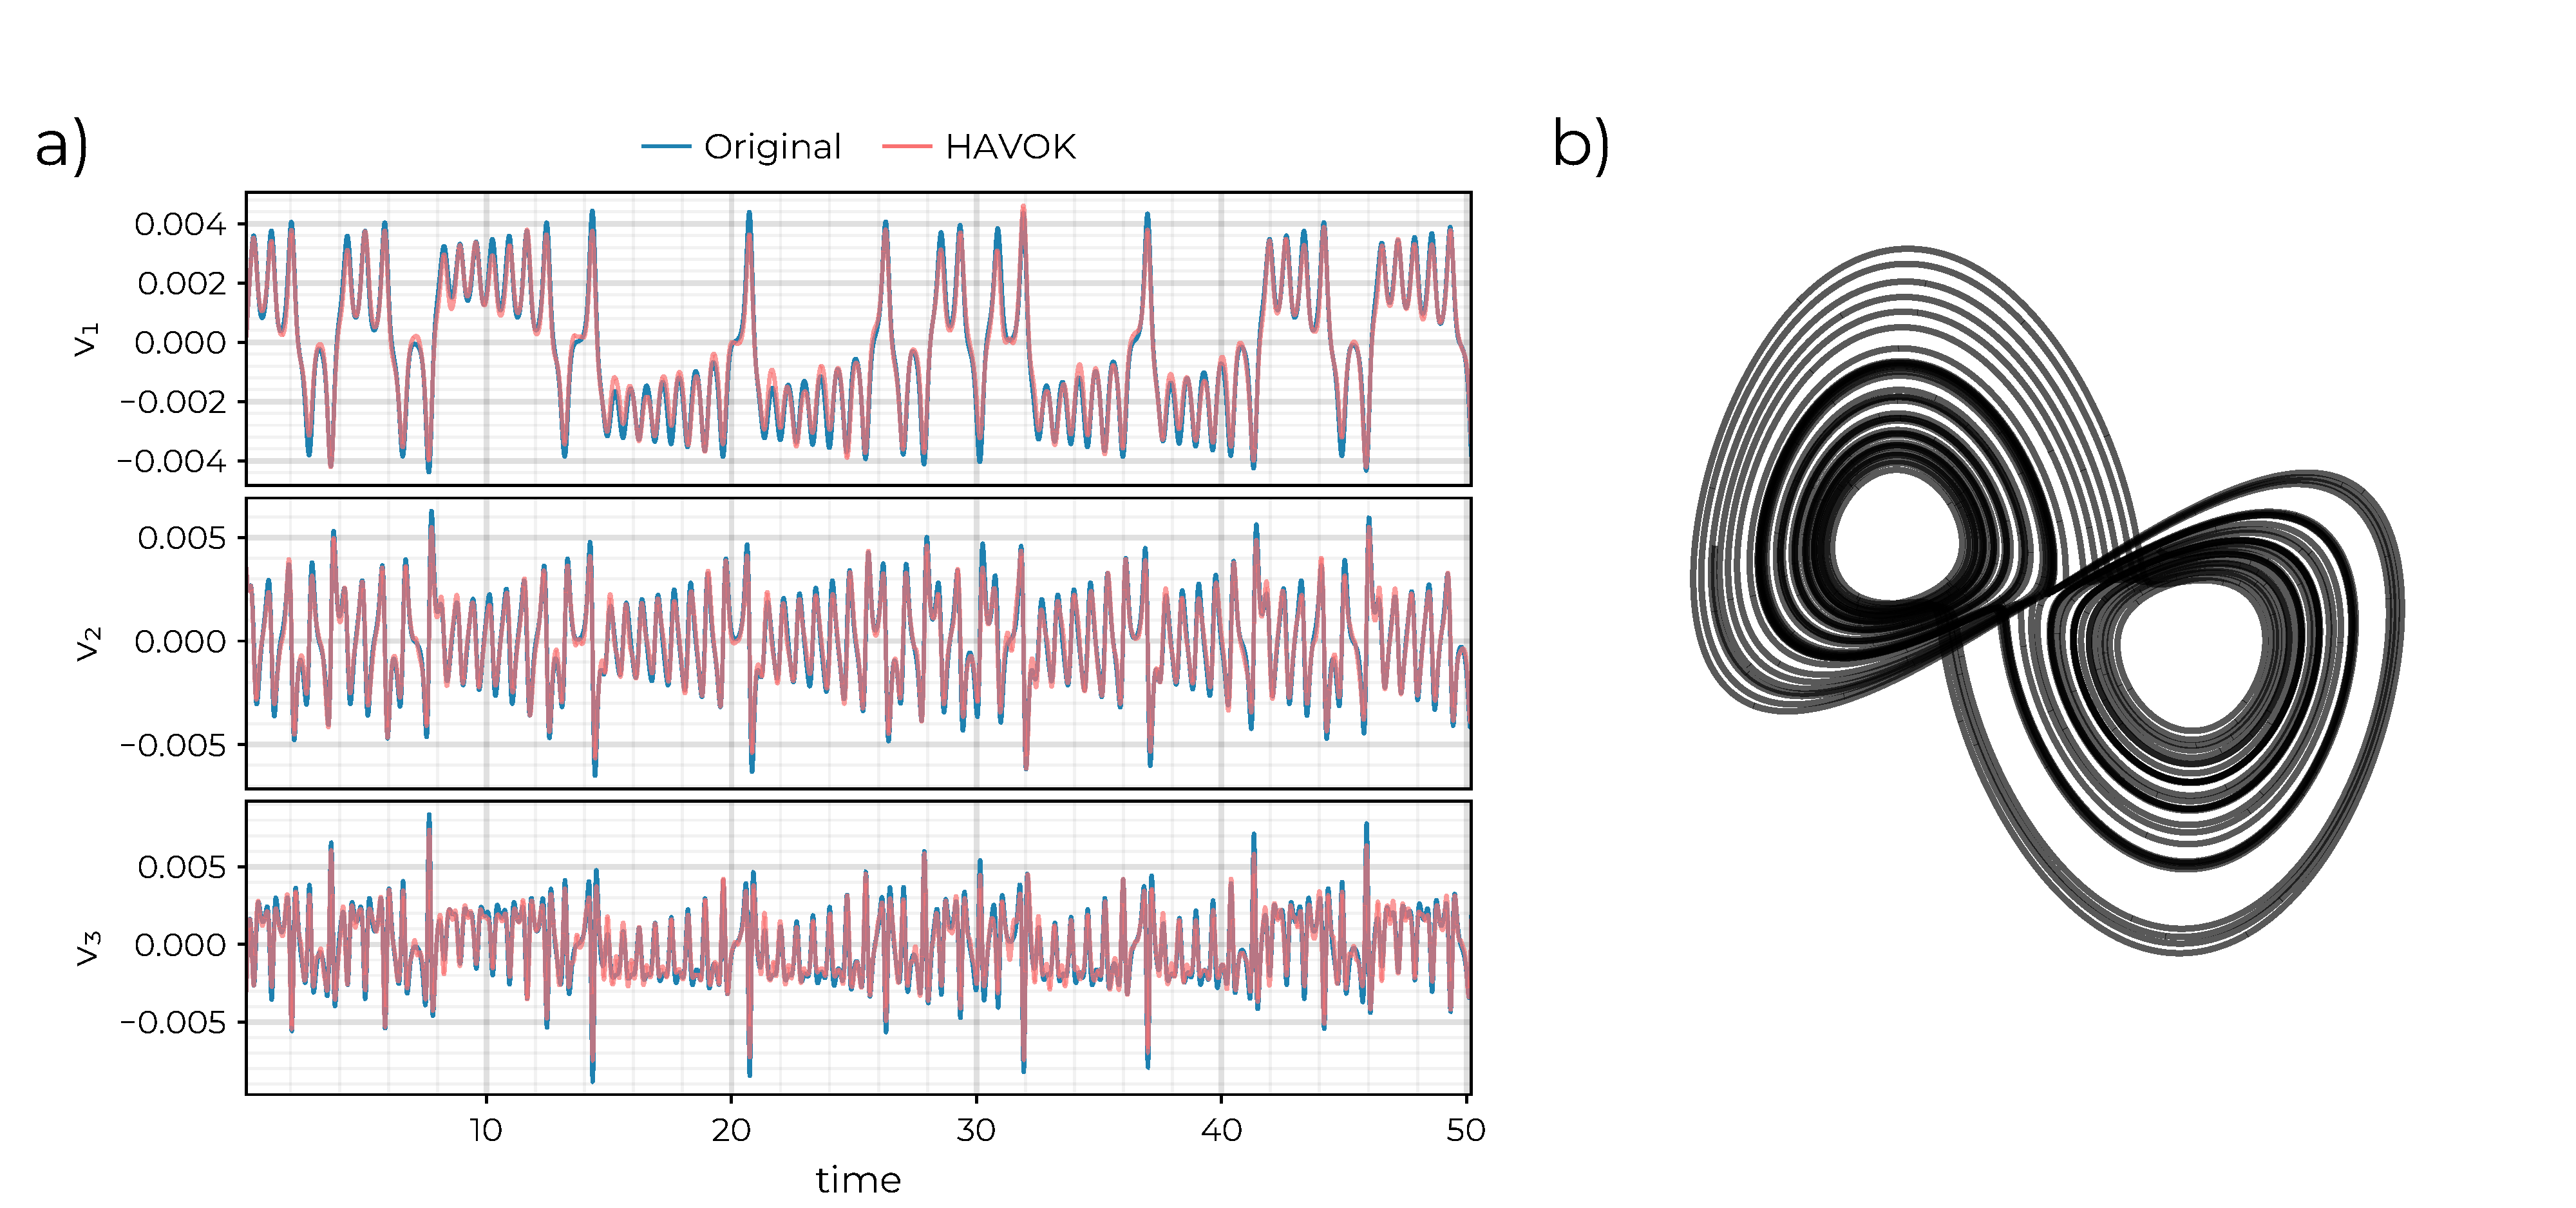
\includegraphics[width=\columnwidth]{havok/0-havok-lorenz/3__havok-embedding.pdf}
  \caption{(\textbf{a}) Time series for first 3 components $v\_i$ of the HAVOK
    model. Original time series for each component are shown in blue. Time
    series predicted by the HAVOK model are overlaid in red. (\textbf(b)) The
    attractor formed by the first 3 embedding coordinates. By Taken's theorem,
    this attractor is diffeomorphic to the original attractor.}
  \label{fig:lorenz-havok-embedding}
\end{figure}



\begin{figure}[h]
  \centering
  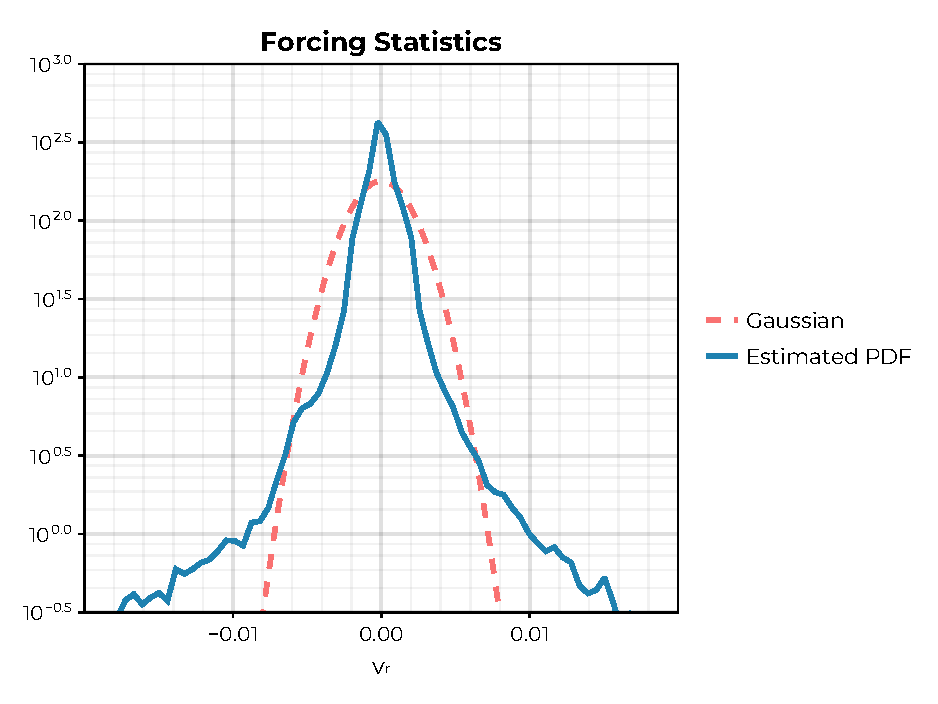
\includegraphics[width=0.75\columnwidth]{havok/0-havok-lorenz/6__forcing-statistics.pdf}
  \caption{Proabability density function for forcing time series learned by the
    HAVOK model. The PDF is compared to a Gaussian fit for the same data. The
    wide tails of the PDF reflect that the forcing is intermittent.}
  \label{fig:lorenz-forcing-stats}
\end{figure}


\begin{figure}[h]
  \centering
  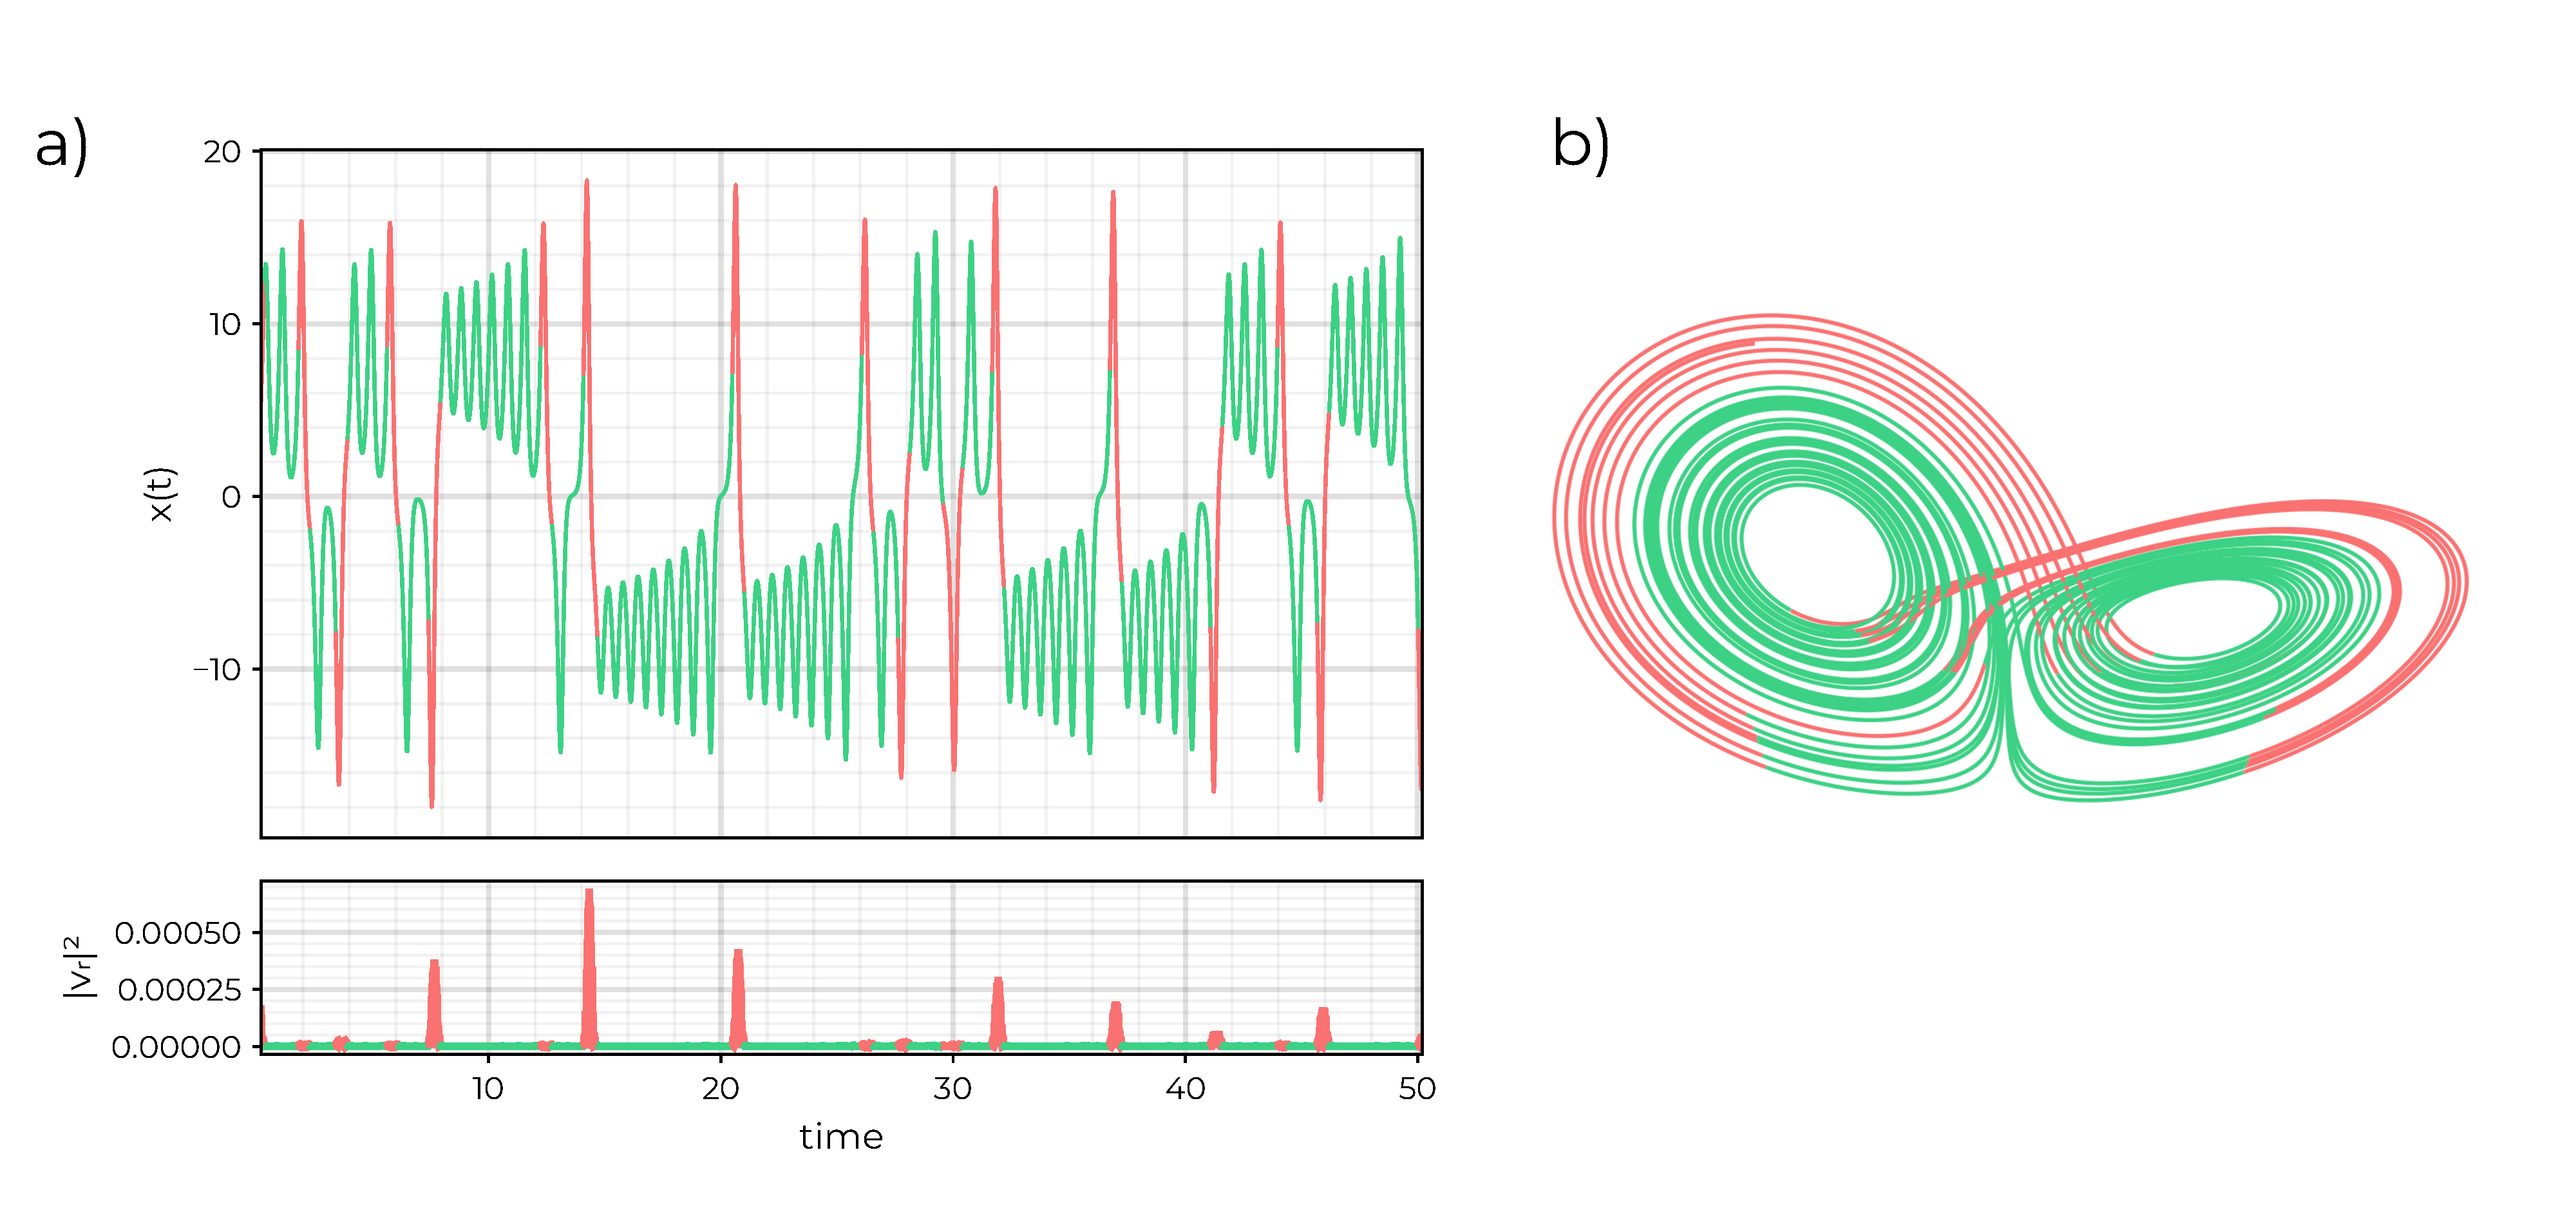
\includegraphics[width=\columnwidth]{havok/0-havok-lorenz/7__attractor-w-forcing.pdf}
  \caption{(\textbf{a}) The original time series $x(t)$ plotted with the squared
  forcing time series $v_r(t)$. Red colors indicate forcing above a chosen
  threshold which accurately identify lobe-switching events. (\textbf{b}) The
  Lorenz attractor colored using the same scheme.}
  \label{fig:lorenz-attractor-forcing}
\end{figure}



\begin{figure}[h]
  \centering
  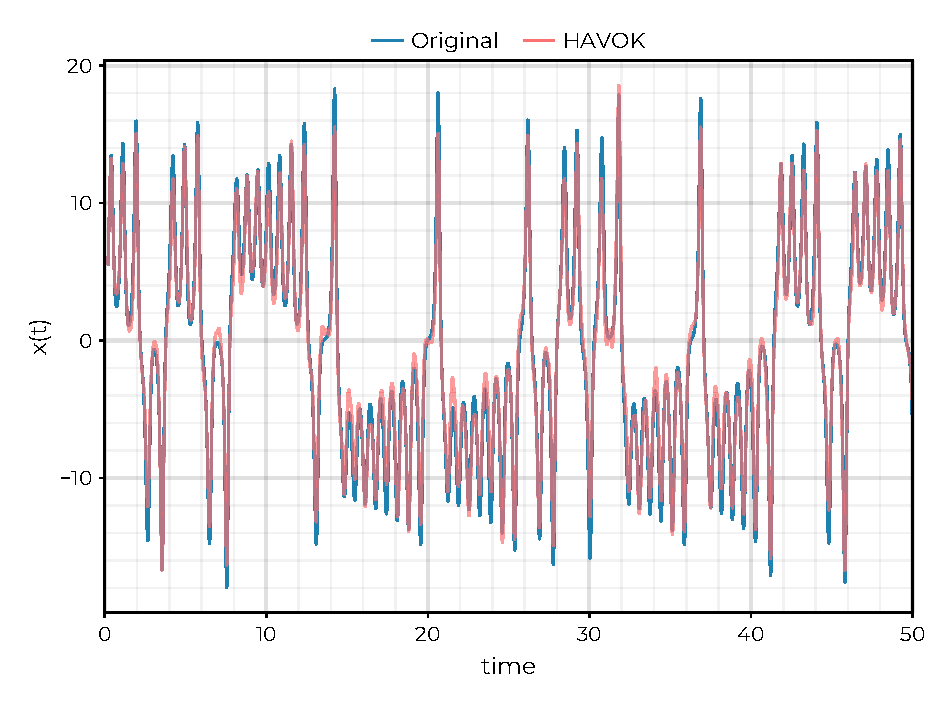
\includegraphics[width=0.9\columnwidth]{havok/0-havok-lorenz/9__timeseries-reconstruction.pdf}
  \caption{The reconstructed time series for $x(t)$ using the learned HAVOK model.}
  \label{fig:lorenz-reconstruction}
\end{figure}




\section{Study Overview}

- Describe dataset, e.g. the specific central node, focus on PM 2.5, and the
collection period (find continuous data during no-rain period during the summer
of 2023 to evaluate HAVOK model independent of problems introduced by
hygroscopic growth)


\begin{figure}[h]
  \centering
  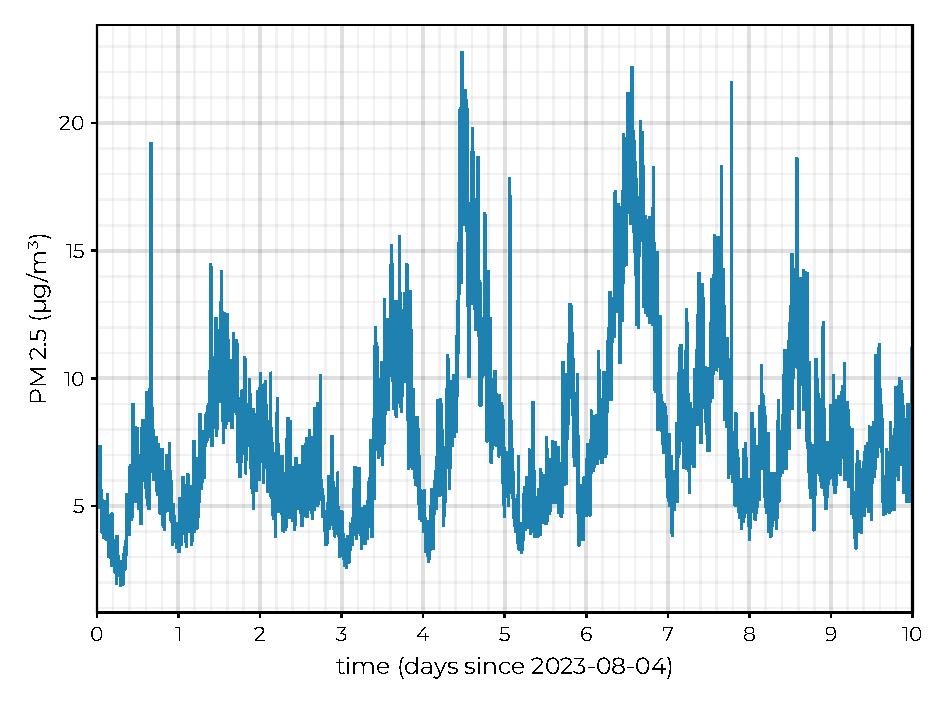
\includegraphics[width=0.8\columnwidth]{havok/1-havok-pm/1__timeseries-full-short.pdf}
  \caption{Time series of PM $2.5$ measurements from Central Hub 4 located in
    Planeo, Tx starting on 2023-08-04. This time series was selected during the
    long period of no precipitation during 2023 in order to limit the impact of
    hygroscopic growth on observed values. Note the occasional, thin vertical
    spikes corresponding to acute pollution events.}
  \label{fig:pm-timeseries-orig}
\end{figure}


\begin{figure}[h]
  \centering
  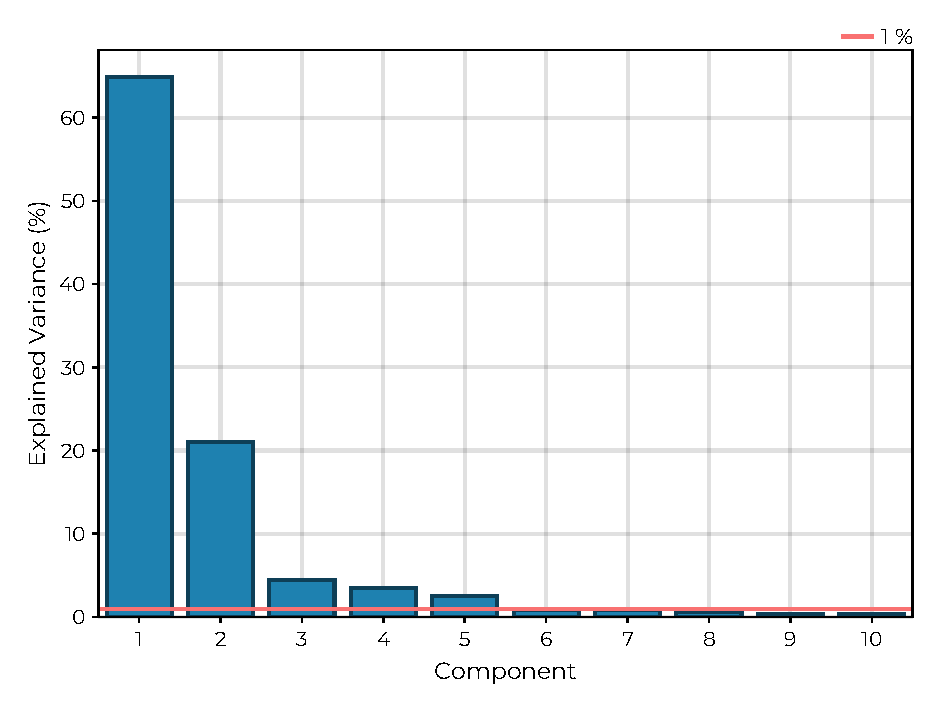
\includegraphics[width=0.7\columnwidth]{havok/1-havok-pm/1__pca-explained-variance.pdf}
  \caption{Explained variance of components from a principal component
    decomposition of the PM 2.5 time series sorted in decreasing order. A red
    line is superimposed indicating a $1\%$ explained variance. All components
    past the sixth contribute less than $1\%$ to the total explained variance. }
  \label{fig:pm-timeseries-pca}
\end{figure}


\section{Results}


\begin{figure}[h]
  \centering
  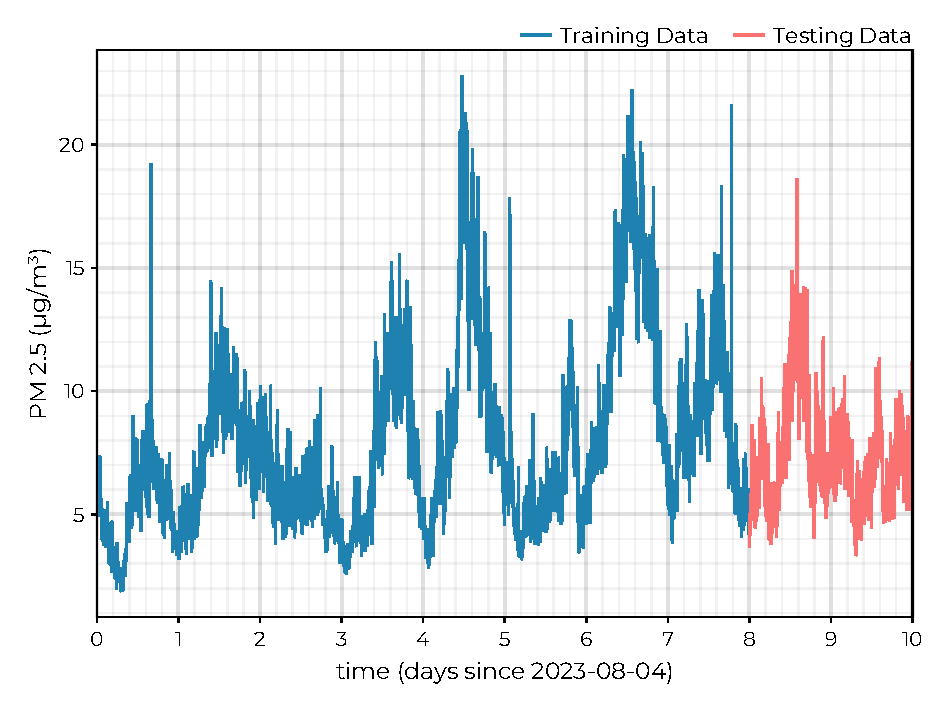
\includegraphics[width=0.8\columnwidth]{havok/1-havok-pm/1b__train-test-timeseries-short.pdf}
  \caption{Train-test split used for training the HAVOK model. To prevent data
    leaks, i.e. information from the future being incorporated into forecasts,
    the data was partitioned into two continuous sets to be used separately for
    model fitting and evaluation.}
  \label{fig:pm-train-test-split}
\end{figure}



\begin{table}[h]
  \caption{Results of HAVOK model hyperparameter search. Models were trained
    varying the embedding size ($N$), number of state variables $(r)$, and
    number of forcing terms ($n$). The top 10 models are presented here as
    evaluated by their RMSE and MAE values ranked in descending order.
    Additionally the top 3 models with $n=1$ are included for comparison.}
  \label{tab:havok-fit-results}
  \centering
  \begin{tabular}{ccccc} \hline
    \textbf{N} & \textbf{r} & \textbf{n} & \textbf{RMSE}  & \textbf{MAE} \\ \hline
    $30$ & $6$ & $5$ & $0.216703$ & $0.155912$ \\
    $45$ & $10$ & $5$ & $0.3649$ & $0.268842$ \\
    $30$ & $6$ & $4$ & $0.472797$ & $0.397746$ \\
    $45$ & $8$ & $5$ & $0.487448$ & $0.358938$ \\
    $30$ & $7$ & $5$ & $0.583654$ & $0.518485$ \\
    $30$ & $8$ & $5$ & $0.58551$ & $0.428986$ \\
    $30$ & $7$ & $4$ & $0.586575$ & $0.520145$ \\
    $30$ & $8$ & $4$ & $0.610296$ & $0.447673$ \\
    $30$ & $8$ & $3$ & $0.620928$ & $0.455369$ \\
    $60$ & $12$ & $5$ & $0.697797$ & $0.507499$ \\
    $\vdots$ & $\vdots$ & $\vdots$ & $\vdots$ & $\vdots$ \\
    $105$ & $3$ & $1$ & $1.48989$ & $1.09792$  \\
    $120$ & $3$ & $1$ &  $1.58473$ & $1.1494$ \\
    $180$ & $5$ & $1$ & $1.77659$ & $1.29506$ 
  \end{tabular}
\end{table}



\begin{figure}[h]
  \centering
  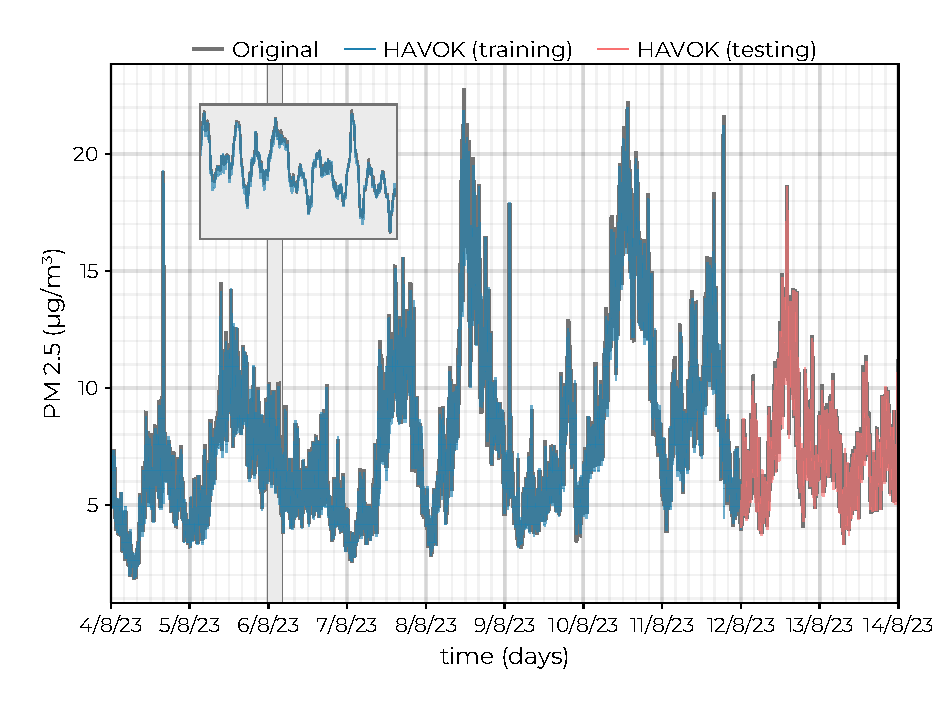
\includegraphics[width=0.75\columnwidth]{havok/2-havok-eval/1__predicted-ts-training.pdf}
  \caption{Time series predicted by HAVOK model with forcing functions provided.
  Inset into the figure is a subset of the }
  \label{fig:pm-havok-predictions}
\end{figure}




\begin{figure}[h]
  \centering
  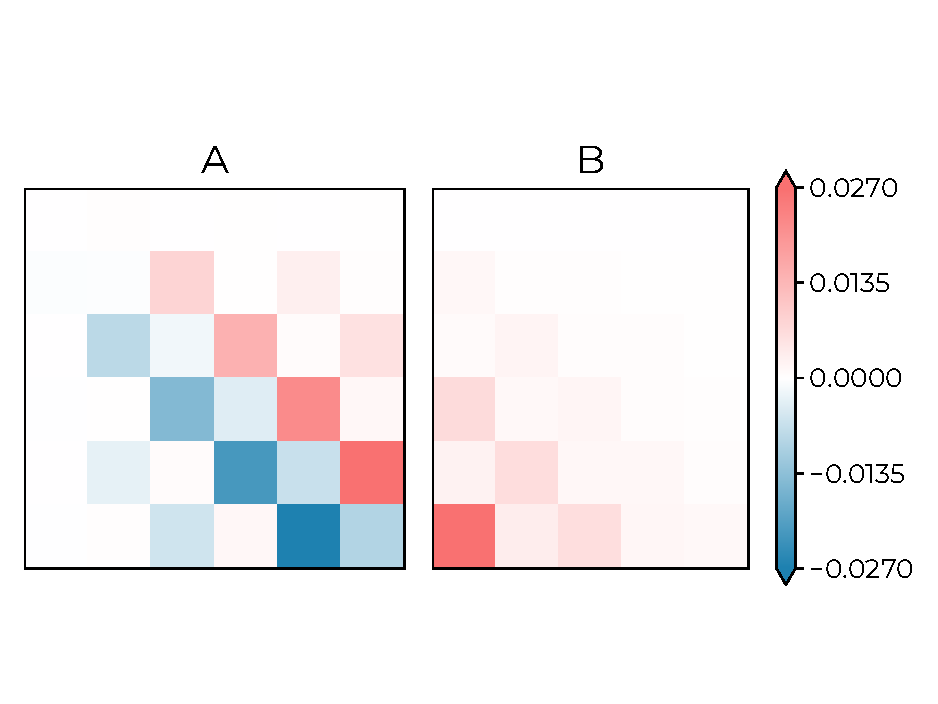
\includegraphics[width=0.65\columnwidth]{havok/2-havok-eval/2__A-B-Havok.pdf}
  \caption{Operators learned by the HAVOK model with $r=6$ and $n=5$. We note
    that the $\mathbf{A}$ matrix displays the expected banded diagonal
    structure. Additionally, the values of the forcing matrix $\mathbf{B}$
    decrease with each column}
  \label{fig:pm-havok-operators}
\end{figure}



\begin{figure}[h]
  \centering
  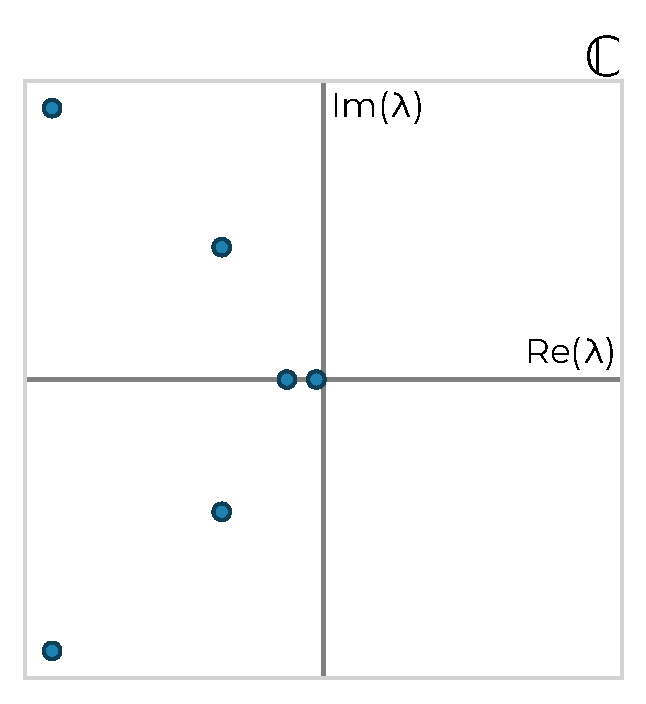
\includegraphics[width=0.35\columnwidth]{havok/2-havok-eval/3__A-eigvals.pdf}
  \caption{Eigenvalues of the learned HAVOK operator $\mathbf{A}$ visualized in
    the complex plane. We note that no eigenvalues had any postive real
    component reflecting the model's stability for integration over long time periods. }
  \label{fig:pm-havok-eigvals}
\end{figure}



\begin{figure}[h]
  \centering
  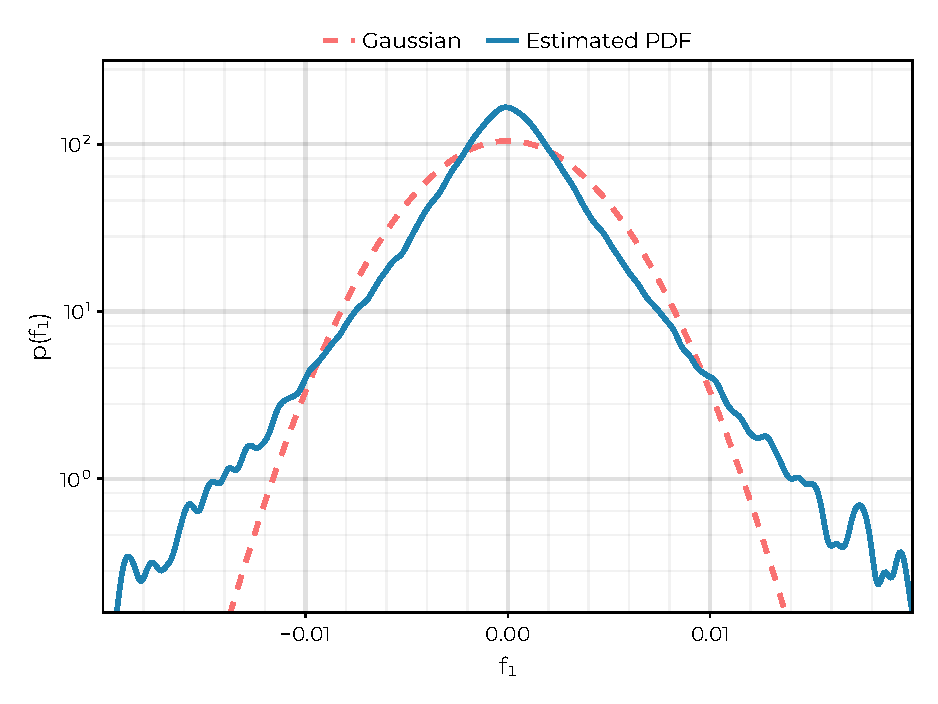
\includegraphics[width=0.65\columnwidth]{havok/2-havok-eval/4__forcing-statistics.pdf}
  \caption{Probability density function evaluated for the first forcing function
  compared to a zero-mean Gaussian distribution fit to the forcing data. The
  wide tails of the estimated distribution reflect the intermittent activation
  of forcing.}
  \label{fig:pm-forcing-stats}
\end{figure}


\begin{figure}[h]
  \centering
  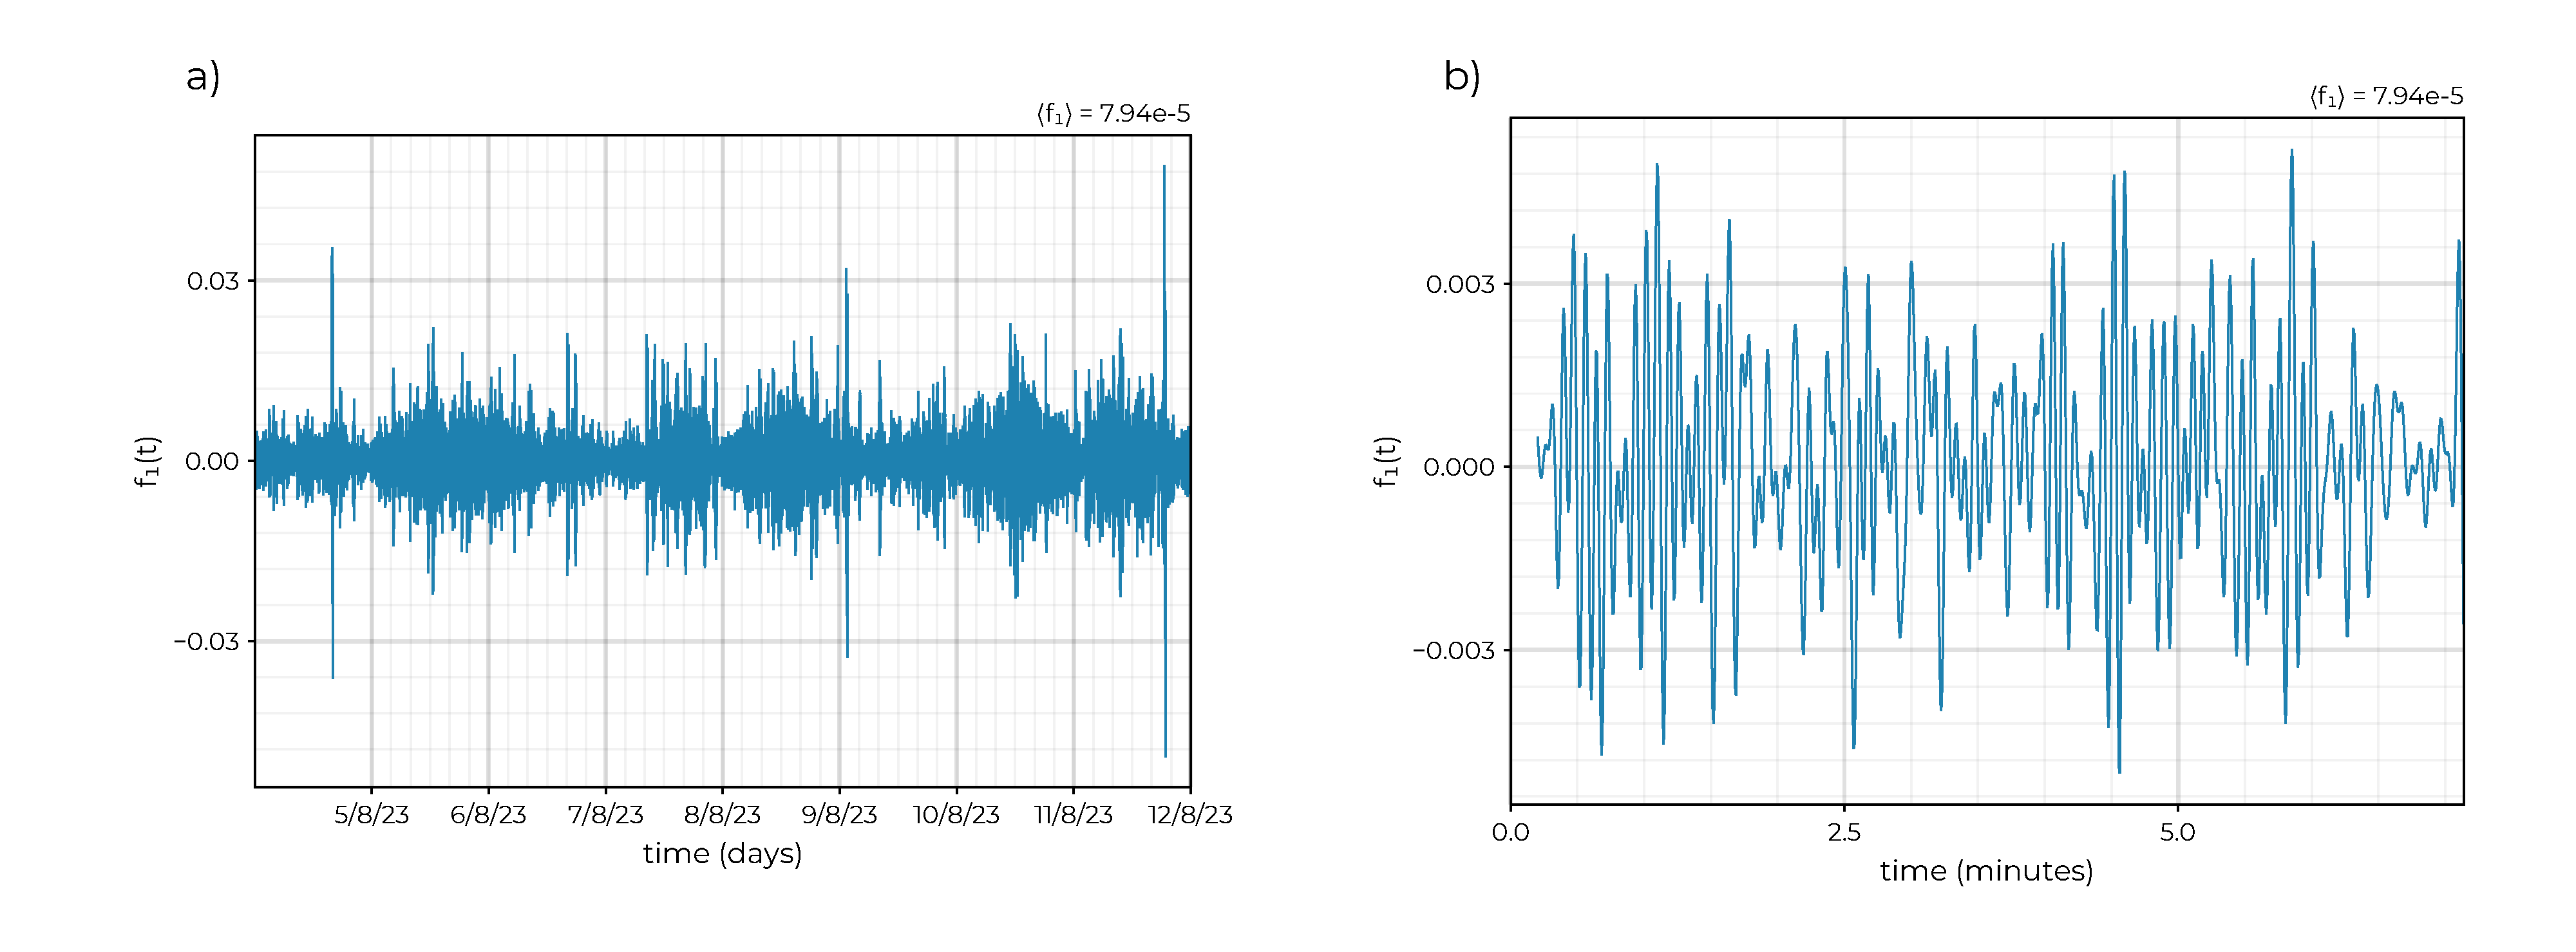
\includegraphics[width=\columnwidth]{havok/2-havok-eval/forcing-time-series.pdf}
  \caption{(\textbf{a}) Time series of first forcing function activation for the
    duration of the training set. (\textbf{b}) The same time series zoomed in to
    the first hours. The mean value for the forcing function was $7.94\times
    10^5$ reflecting the fact that the learned forcing functions tend to be
    centered about zero with no long-term trend.}
  \label{fig:pm-forcing-time-series}
\end{figure}


\begin{figure}[h]
  \centering
  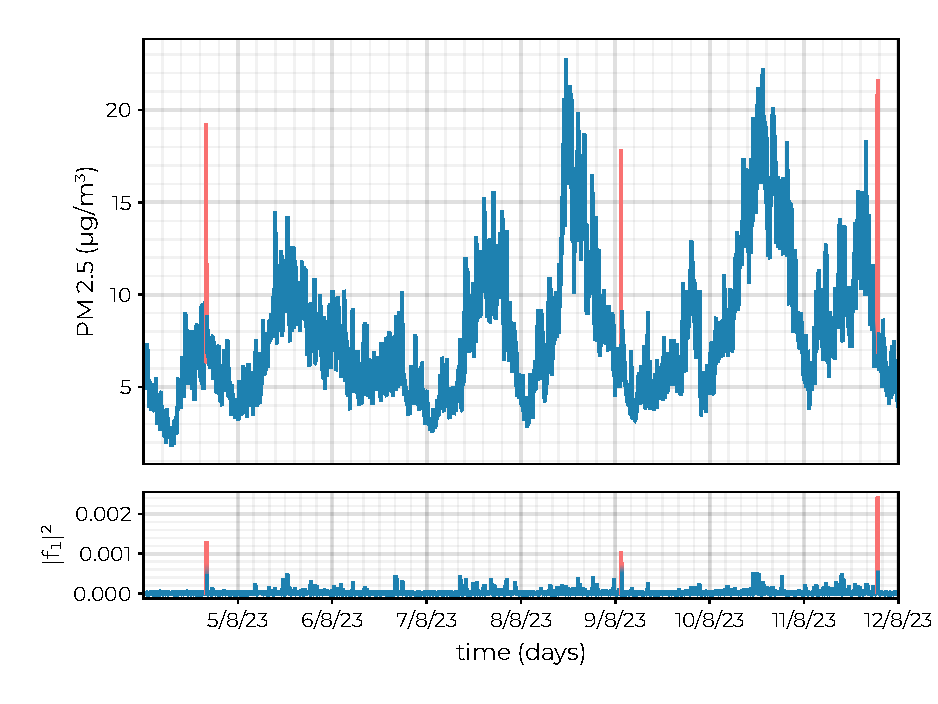
\includegraphics[width=\columnwidth]{havok/2-havok-eval/6__timeseries-with-forcing.pdf}
  \caption{The original PM 2.5 time series plotted together with the squared
    value of the first forcing function, $\lVert  f_1(t) \rVert^2$. By
    thresholding the values of $f_1$, the intermittent PM spikes are easily
    identified. }
  \label{fig:pm-time-series-w-forcing}
\end{figure}




\begin{table}[h]
  \caption{Evaluation of HAVOK forecasting performance as a function of
    prediction horizon from 10 seconds to 4 minutes.}
  \label{tab:havok-forecasting-results}
  \centering
  \begin{tabular}{ccccccc} \hline
    \textbf{Duration} & \textbf{RMSE}  & \textbf{RMSE} & \textbf{MAE}   & \textbf{MAE}  & \textbf{MAPE}  & \textbf{MAPE} \\
                      & \textbf{train} & \textbf{test} & \textbf{train} & \textbf{test} & \textbf{train} & \textbf{test} \\\hline
    10 sec.	  & 0.0611 & 0.0589 & 0.0415 & 0.0415 & 0.0054 & 0.0057 \\
    1 min.	  & 0.2555 & 0.2398 & 0.1757 & 0.1720 & 0.0231 & 0.0235 \\
    2 min.	  & 0.7056 & 0.6764 & 0.4874 & 0.4945 & 0.0640 & 0.0674 \\
    3 min.	  & 1.0552 & 1.0366 & 0.7290 & 0.7691 & 0.0957 & 0.1052 \\
    4 min.	  & 1.3759 & 1.3567 & 0.9530 & 1.0185 & 0.1252 & 0.1389 \\
    5 min. 	  & 1.6696 & 1.6530 & 1.1611 & 1.2475 & 0.1525 & 0.1703
  \end{tabular}
\end{table}






\begin{figure}[h]
  \centering
  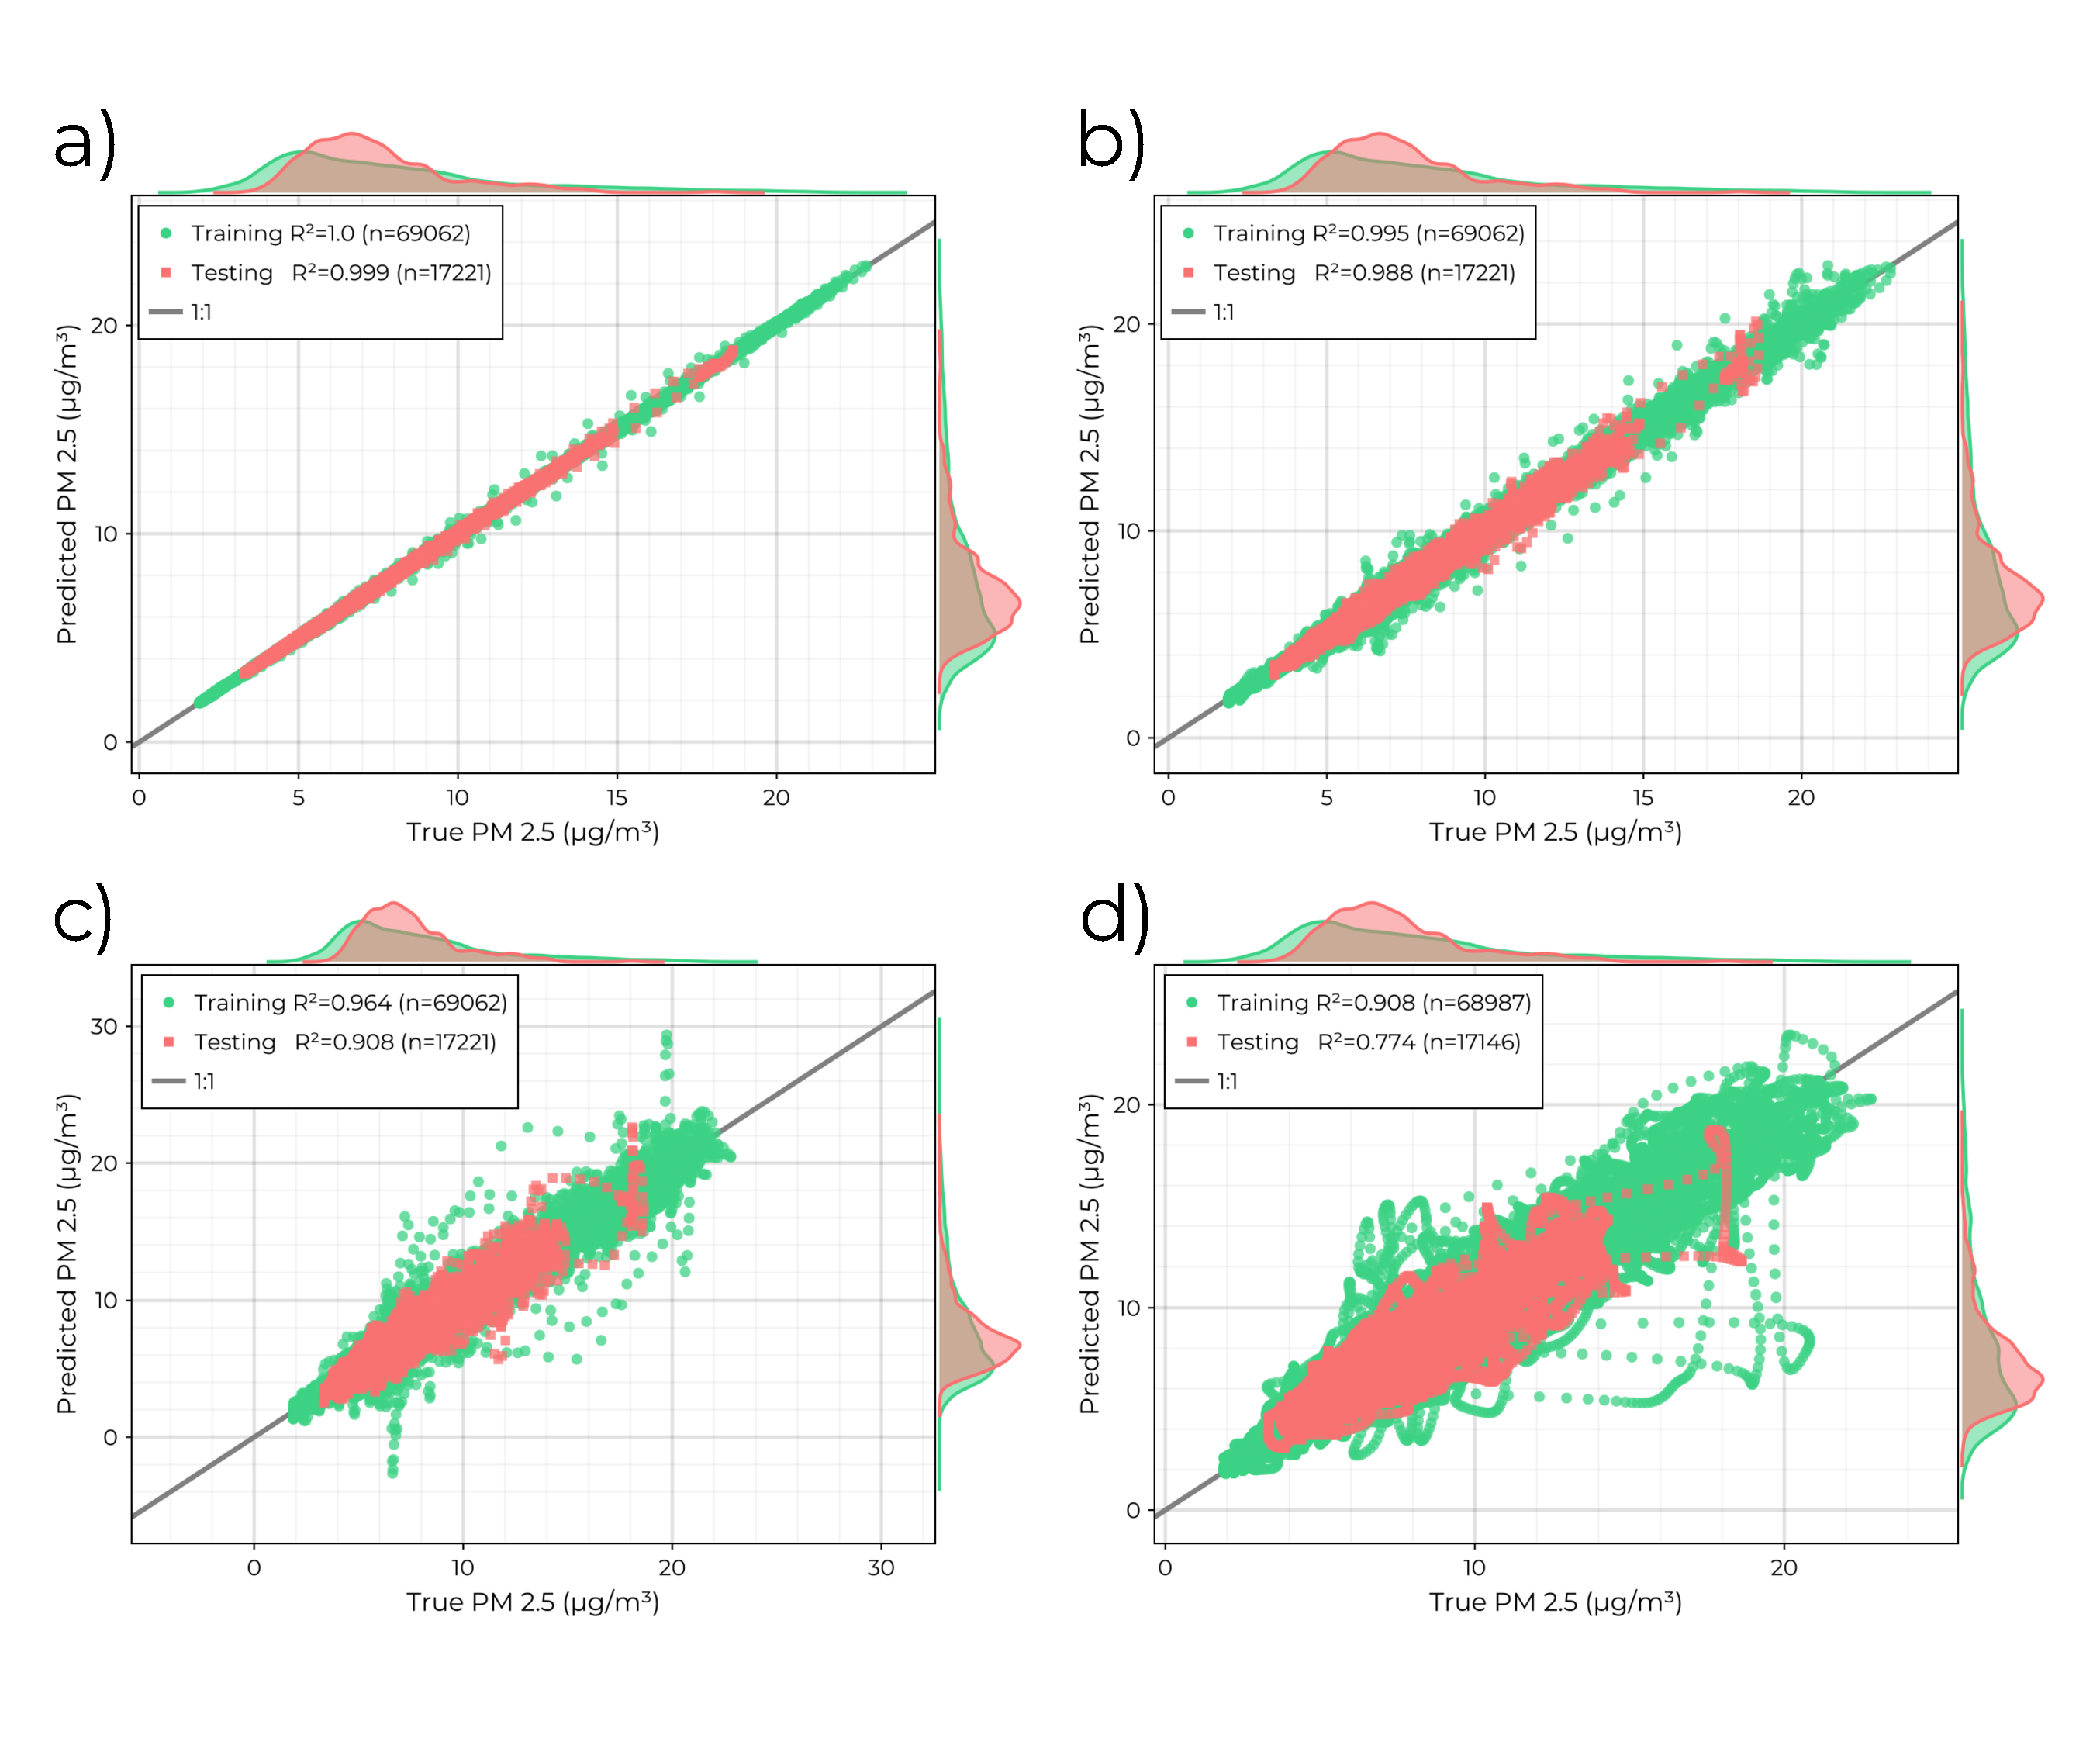
\includegraphics[width=\columnwidth]{havok/3-forcing-fit/forecast-scatter.pdf}
  \caption{Scatter diagrams for multistep forecasts. (\textbf{a}) 10 second
    forecast. (\textbf(b)) 1 minute forecast. (\textbf{c}) 2 minute forecast.
    (\textbf{d}) 5 minute forecast. The integration time step was $\Delta t =
    10$ s so that a 5 minute forecast corresponds to a 30 step future prediction.}
  \label{fig:pm-time-series-w-forcing}
\end{figure}

